\chapter{Сравнение аукционов в общем случае}

%Если вы будете читать Сергея Николенко, то осторожно, там есть несколько опечаток со знаками неравенств.


Сравним доходность трёх аукционов (первой, второй цены и кнопочного) для продавца в общем случае. Предположений у нас будет всего два: аффилированность сигналов и симметричность игроков.

\section{Про симметричность}
Для наглядности приведём три примера впереди определения:

\begin{myex} Совместная функция плотности сигналов имеет вид:
\begin{equation}
f(x_{1},x_{2},x_{3})=\frac{7}{8}+x_{1}x_{2}x_{3}
\end{equation}
Ценности определяются по формулам:
\begin{equation}
\begin{array}{c}
V_{1}=X_{1}+\sqrt{X_{2}X_{3}+1}-1 \\
V_{2}=X_{2}+\sqrt{X_{1}X_{3}+1}-1 \\
V_{3}=X_{3}+\sqrt{X_{1}X_{2}+1}-1
\end{array}
\end{equation}
Всё симметрично. Ценность товара для меня может по-особому зависеть от моего сигнала, но должна одинаково зависеть от сигнала других игроков. С моей точки зрения другие игроки одинаковые, и то, что знают они, чего не знаю я, должно одинаково воздействовать на ценность товара для меня.
\end{myex}


\begin{myex} Совместная функция плотности сигналов имеет вид
\begin{equation}
f(x_{1},x_{2},x_{3})=x_{1}\left(\frac{7}{8}+\frac{1}{2}x_{2}x_{3}\right)
\end{equation}
Ценности определяются по формулам
\begin{equation}
\begin{array}{c}
V_{1}=X_{1}+\sqrt{X_{2}X_{3}+1}-1 \\
V_{2}=X_{2}+\sqrt{X_{1}X_{3}+1}-1 \\
V_{3}=X_{3}+\sqrt{X_{1}X_{2}+1}-1
\end{array}
\end{equation}
Несимметрична функция плотности.
\end{myex}

\begin{myex} Совместная функция плотности сигналов имеет вид
\begin{equation}
f(x_{1},x_{2},x_{3})=\frac{7}{8}+x_{1}x_{2}x_{3}
\end{equation}
Ценности определяются по формулам:
\begin{equation}
\begin{array}{c}
V_{1}=X_{1}+\sqrt{X_{2}X_{3}+1}-1 \\
V_{2}=X_{2}+X_{3} \\
V_{3}=X_{3}\cdot X_{1} \\
\end{array}
\end{equation}
Несимметричны ценности.
\end{myex}

Для формальности:
\begin{mydef}
Функция $ f(a,b,c,d,e) $ симметрична относительно аргументов $ a,b,c $, если её значение не изменится при перестановке $ a$, $b$  и $c$ в другом порядке.\index{симметричная функция}
\end{mydef}

\begin{myex} Функция симметричная относительно $ x $ и $ y $: $ f(x,y,z)=xy+z $
\end{myex}

\begin{myex} Функция симметричная относительно всех аргументов:
$$ f(w,x,y,z)=xyz+wxy+wxz+wyz $$
\end{myex}


\begin{mydef} Игроков будем называть \indef{симметричными}\index{симметричные игроки}, если:
\begin{enumerate}
\item Совместная функция плотности $ f(x_{1},x_{2},\ldots,x_{n}) $ симметрична по всем аргументам
\item Ценность $V_{i}$ определяется по формуле:
\begin{equation}
V_{i}=u(X_{i},X_{-i})
\end{equation}
где: $X_{-i}  $ — это вектор $ (X_{1},X_{2},\ldots,X_{n}) $, в котором отсутствует $ X_{i} $, а  функция $ u(t,t_{1},t_{2},\ldots,t_{n-1}) $ симметрична по аргументам $ t_{1} $,\ldots, $ t_{n-1} $, то есть по всем аргументам, кроме первого аргумента $ t $.

\end{enumerate}
\end{mydef}

\subsubsection*{Предпосылки на функцию полезности}\index{предпосылки на функцию полезности}
Кроме того, функция полезности $ u() $ удовлетворяет условиям:
\begin{enumerate}
\item Не убывает по всем аргументам. Это означает, что сигнал $ X_{i} $ положительно связан с ценностью.
\item Отмасштабирована так, что $ u(0,0,\ldots,0)=0 $. Это просто условие нормировки. Если все получили сигнал «Товар просто никакой», значит, товар действительно никакой.
\end{enumerate}






\section{Ещё об аффилированности}


Сперва кое-что о вероятностях\ldots

Если у нас есть случайная величина $ Z $, то мы можем построить функцию $z(y)= \E(Z|Y=y) $. Рассмотрим эту функцию в случайной точке $ Y $:
\begin{multline}
\E(z(Y))=\int_{0}^{1}z(y)f_{Y}(y)dy=\int_{0}^{1}\int_{0}^{1}z\cdot \frac{f(y,z)}{f_{Y}(y)}dz f_{Y}(y)dy=\\
=\int_{0}^{1}\int_{0}^{1}z\cdot f(y,z)dydz=\E(Z)
\end{multline}

Значит, это нам это даёт способ расчёта $ \E(Z) $:\index{условное математическое ожидание}
\begin{equation}
\label{conditional_way}
\E(Z)=\int_{0}^{1}\E(Z|Y=y)f_{Y}(y)dx
\end{equation}

Честно говоря, этот способ мы уже использовали. Он очень мощный.

Если глубоко копать, то можно понять, что это не что иное, как теорема о трёх перпендикулярах\index{теорема!о трёх перпендикулярах} из 11-го класса средней школы. Математическое ожидание случайной величины — это её проекция на множество действительных чисел. Квадратом расстояния между двумя случайными величинами при этом служит $ \E((X-Y)^{2}) $. Например, теорема Пифагора формулируется так: $ \E(X^{2})=\E(m^{2})+\E((X-m)^{2}) $. Три перпендикуляра: наклонная — это $ Y $; плоскость — это множество случайных величин, записывающихся как функция от $ X $; проекция на плоскость — это функция $ \E(Y|X=x) $, взятая в случайной точке $ X $; множество констант — это прямая в нашей плоскости; $ \E(Y) $ — это проекция на прямую\ldots


% #TODO: картинка для условного ожидания

Аналогично, довесив условие $X=x$ слева и справа, можно получить, что
\begin{equation}
\label{iterated_e}
\E(Z|X=x)=\int_{0}^{1}\E(Z|Y=y, X=x)f_{Y|X}(y|x)dy
\end{equation}

Это не очевидно. Те, кому интересна теория вероятностей могут вывести это утверждение, остальные могут поверить.

Теперь вернемся к аффилированности.

\begin{myth}
\label{aff_order}
Если величины $ X_{1} $, \ldots, $ X_{n} $ аффилированы, то и величины $ X_{1} $, $ Y_{1} $, $ Y_{2} $, \ldots, $ Y_{n-1} $ аффилированы. \index{аффилированные случайные величины}\index{теорема!об аффилированных случайных величинах}
\end{myth}

\begin{proof}
Великие о-малые говорят нам, что совместная функция плотности вектора $ X_{1} $, $ Y_{1} $, $ Y_{2} $, \ldots, $ Y_{n-1} $ на участке $ y_{1}>y_{2}>\ldots>y_{n-1} $ равна\index{о-малые}
\begin{equation}
f_{X_{1},Y_{1},\ldots,Y_{n-1}}(x_{1},y_{1},y_{2},\ldots,y_{n-1})=(n-1)!f(x_{1},y_{1},\ldots,y_{n-1})
\end{equation}
Нам нужно проверить супермодулярность логарифма,
\begin{equation}
\ln(f_{X_{1},Y_{1},\ldots,Y_{n-1}}(x_{1},y_{1},y_{2},\ldots,y_{n-1}))=\ln((n-1)!)+\ln(f(x_{1},y_{1},\ldots,y_{n-1}))
\end{equation}

Вторые смешанные производные от левой части неотрицательны в силу того, что неотрицательны вторые смешанные производные от правой части.

\end{proof}



Теоремы, которые мы далее докажем, будут верны для любых аффилированных случайных величин. Но мы будем иметь ввиду величины $ X_{1} $ и $ Y_{1} $, поэтому будем использовать соответствующие обозначения.

\begin{myth}
\label{aff_delete}\index{теорема!об аффилированных случайных величинах}
Если из набора аффилированных величин некоторые удалить, то оставшиеся будут аффилированы.
\end{myth}

\begin{proof}
Здесь приведём только подсказку к доказательству. Достаточно доказать, что набор остаётся аффилированым, если удалить из него одну случайную величину. Удалять поднабор величин можно последовательно по одной. \end{proof}


Из теорем \ref{aff_delete} и \ref{aff_order} следует, что $ X_{1} $ и $ Y_{1} $ аффилированы. Для трёх аукционов, которые мы сравниваем, знание этих двух величин позволяет определить, победил ли первый игрок, и сколько он платит.

Нам надо изучать величины $ X_{1} $ и $ Y_{1} $, но, чтобы постоянно не писать индекс $ _{1} $ в доказательствах, пока забудем про него.

Введём несколько обозначений для этой пары:
\begin{enumerate}
\item $ g(x,y) $ — их совместная функция плотности,
\item $ g(y|x)=\frac{g(x,y)}{f_{X}(x)} $ — условная функции плотности $ Y $ при заданном $ X $
\item $ G(y|x)=\P(Y\leq y|X=x)$ — условная функции распределения $ Y $ при заданном $ X $.

Конечно, верно соотношение:
\begin{equation}
G(y|x)=\P(Y\leq y|X=x)=\int_{0}^{y}g(t|x) \, dt
\end{equation}

\item $ R(y|x)=\frac{g(y|x)}{G(y|x)} $ — условная обратная функция риска\index{условная обратная функция риска} $ Y $ при заданном $ X $.

Поясним её смысл. Это шансы того, что $ Y $ будет около $ y $, если известно, что $ Y\leq y $ и $ X=x $. Например, значение $ R(10,20)=30 $ можно проинтерпретировать так. Возьмем маленький $ \Delta y=0.01 $. Тогда $ \P(Y\in [9.99;10]|Y\leq 10, X=20)\approx 30\cdot 0.01=0.3 $.
\end{enumerate}

При расчете $ R(y|x) $ можно не считать $ f_{X}(x) $, так как оно сокращается:
\begin{equation}
R(y|x)=\frac{g(y|x)}{G(y|x)}=\frac{g(x,y)}{\int_{0}^{y}g(x,t) \, dt}
\end{equation}

Нам потребуется небольшой технический результат:
\begin{myth}\index{теорема!о свойствах аффилированных случайных величин}
Если случайные величины $ X $ и $ Y $ аффилированы, и $ g(x,y) $ — их совместная функция плотности, то\footnote{Тут обычно в учебниках вводят кучу определений (стохастическое доминирование, доминирование в терминах обратной доли риска и пр.), но мы не будем этого делать.}
\begin{enumerate}
\item условная функция распределения $ G(y|x)$ — не возрастает по $ x $\index{условная функция распределения},
\item условная обратная функция риска  $ R(y|x)=\frac{g(y|x)}{G(y|x)} $ — не убывает по $ x $.\index{условная обратная функция риска}
\end{enumerate}
\end{myth}
\begin{proof}
Величины $ X $ и $ Y $ аффилированы.

Рассмотрим пару точек $ (x',y) $ и $ (x,y') $. Воспользуемся аффилированностью,
\begin{equation}
g((x',y)\wedge (x,y'))\cdot g((x',y)\vee (x,y'))\geq g(x',y)\cdot g(x,y')
\end{equation}


Пусть $ x'\geq x $ и $ y'\geq y $. Тогда
\begin{equation}
g(x,y)\cdot g(x',y')\geq g(x',y)\cdot g(x,y')
\end{equation}

Поскольку $ g(x,y)=g(y|x)\cdot f_{X}(x) $ мы получаем, что
\begin{equation}
g(y|x)\cdot f_{X}(x)\cdot g(y'|x')\cdot f_{X}(x')\geq g(y|x')\cdot f_{X}(x')\cdot g(y'|x)\cdot f_{X}(x)
\end{equation}

Убираем повторы,
\begin{equation}
g(y|x)\cdot g(y'|x')\geq g(y|x')\cdot g(y'|x)
\end{equation}

Или
\begin{equation}
\frac{g(y|x)}{g(y'|x)}\geq \frac{g(y|x')}{g(y'|x')}
\end{equation}

Интегрируем по $ y $ от $ 0 $ до $ y' $,
\begin{equation}
\frac{G(y'|x)}{g(y'|x)}\geq \frac{G(y'|x')}{g(y'|x')}
\end{equation}

Переворачиваем дробь,
\begin{equation}
\frac{g(y'|x)}{G(y'|x)}\leq \frac{g(y'|x')}{G(y'|x')}
\end{equation}

Используя условную обратную функцию риска,
\begin{equation}
R(y'|x)\leq R(y'|x')
\end{equation}

А у нас $ x\leq x' $. Это и означает, что $ R(\cdot|x) $ не убывает по $ x $.

Осталось доказать, что $ G(y'|x) $ не возрастает по $ x $. Мы докажем, что $ \ln (G(y'|x)) $ не возрастает по $ x $.

Заметим, что
\begin{equation}
\frac{\partial \ln (G(y'|x))}{\partial y'}=\frac{g(y'|x)}{G(y'|x)}=R(y'|x)
\end{equation}

Или
\begin{equation}
\ln(G(y'|x))=\int_{1}^{y'}R(t|x)dt
\end{equation}

Обратите внимание, что здесь несколько непривычные пределы интегрирования: не от $0$, а от $ 1 $. Связано это с тем, что интеграл должен обращаться в 0 не при $ y'=0 $, а при $ y'=1 $. Действительно, у нас регулярное распределение на $ [0;1] $, значит, $ G(1|x)=1 $ и $ \ln (G(1|x))=0 $. Заметьте, что знаки при этом совпадают. Cлева отрицательное выражение, так как $ G\in (0;1) $. Справа отрицательное, так как верхний предел меньше нижнего.

Давайте перепишем в привычном варианте, когда верхний предел интегрирования больше нижнего,
\begin{equation}
\ln(G(y'|x))=-\int_{y'}^{1}R(t|x)dt
\end{equation}

С ростом $ x $ подынтегральное выражение растёт для любого $ t $, значит, растёт результат интегрирования. То есть функция $\ln( G(y'|x) )$ не возрастает по $ x $.

\end{proof}









Из этих свойств следует теорема имеющая более наглядный смысл:
\begin{myth} \label{prop_affiliated}
Если $ X $ и $ Y $ аффилированы, то: \index{теорема!об аффилированных случайных величинах}
\begin{enumerate}
\item Функция $ \E(Y|X=x )$ не убывает по $ x $,
\item Если $ \gamma() $ — возрастающая функция, то $ \E(\gamma(Y)|X=x) $ не убывает по $ x $,
\item $\Cov(X,Y)\geq 0 $.
\end{enumerate}
\end{myth}




\begin{proof}
По определению,
\begin{equation}
\E(Y|X=x)=\int_{0}^{1}yg(y|x)dy
\end{equation}

Мы можем проинтегрировать по частям ($ u=y $, $ v'=g(y|x) $) и получить:
\begin{equation}
\E(Y|X=x)=\left.yG(y|x)\right|_{y=0}^{y=1} - \int_{0}^{1}G(y|x) \, dy
\end{equation}

Поскольку мы работаем с регулярным на $ [0;1] $ распределением, то $ G(0|x)=0 $ и $ G(1|x)=1 $. Ещё раз напомню, что выбор 0 и 1 в качестве границ распределения — это просто масштабирование для удобства и все наши доказательства проходят без изменений для случая регулярного распределения на отрезке $ [a;b] $.
\begin{equation}
\E(Y|X=x)=1 - \int_{0}^{1}G(y|x)dy
\end{equation}

Остаётся заметить, что с ростом $ x $ падает подынтегральное выражение и, следовательно, интеграл. Значит, $ \E(Y|x=x) $ возрастает.

Доказательство для произвольной $ \gamma(y) $ ничем не отличается:
\begin{equation}
\E(\gamma(Y)|X=x)=\int_{0}^{1}\gamma(y)g(y|x)dy
\end{equation}

Интегрируя по частям получаем,
\begin{equation}
\E(\gamma(Y)|X=x)=\left.\gamma(y)G(y|x)\right|_{y=0}^{y=1} - \int_{0}^{1}\gamma'(y)G(y|x)dy
\end{equation}

Или
\begin{equation}
\E(\gamma(Y)|X=x)=1 - \int_{0}^{1}\gamma'(y)G(y|x)dy
\end{equation}
Снова замечаем, что с ростом $ x $ падает подынтегральное выражение. Следовательно, функция $ \E(\gamma(Y)|X=x) $ возрастает по $x$.


Теперь про ковариацию. Пусть $ \E(X)=m $. Тогда
\begin{multline}
\Cov(Y,X)=Cov(Y,X-m)=\E(Y(X-m))-\E(Y)\E(X-m)=\\
\E(Y(X-m))-\E(Y)\cdot 0=\E(Y(X-m))
\end{multline}

Пользуемся условным способом расчёта математического ожидания \ref{conditional_way}:
\begin{multline} \index{условное математическое ожидание}
\E(Y\cdot (X-m))=\int_{0}^{1} \E(Y(X-m)|X=x)f_{X}(x)dx=\\
=\int_{0}^{1}\E(Y|X=x)(x-m)f_{X}(x)dx
\end{multline}

Теперь мы замечаем, что если бы не было сомножителя $ \E(Y|X=x) $, то интеграл бы равнялся нулю, так как
\begin{equation}
\int_{0}^{1}(x-m)f_{X}(x)dx=\E(X-m)=\E(X)-m=0
\end{equation}

А теперь глядим на функцию $ (x-m)f_{X}(x) $. Сначала она отрицательна, затем положительна, суммарная площадь под функцией равна нулю

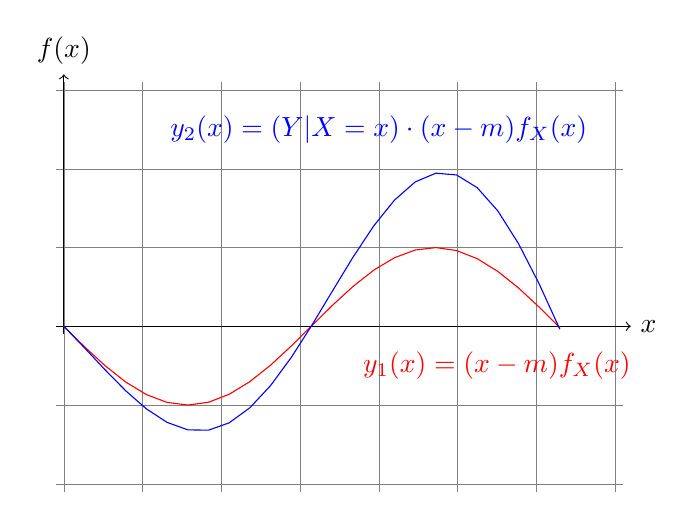
\begin{tikzpicture}[domain=0:6.3]
    \draw[very thin,color=gray] (-0.1,-2.1) grid (7.1,3.1);
    \draw[->] (-0.1,0) -- (7.2,0) node[right] {$x$};
    \draw[->] (0,-0.1) -- (0,3.2) node[above] {$f(x)$};
    \draw[red] plot (\x,{-sin(\x r)});
    \draw[blue] plot (\x, {-(1+\x/5)*sin(\x r)}) ;
    \node[blue] at (4,2.5) {$y_2(x)=\E(Y|X=x)\cdot (x-m)f_X(x)$};
    \node[red] at (5.5,-0.5) {$y_1(x)=(x-m)f_X(x)$};
\end{tikzpicture}

Функция $ \E(Y|X=x) $ положительна и возрастает по $ x $, значит, холм растягивается сильнее, чем яма. Следовательно, равный ковариации интеграл $ \int_{0}^{1}\E(Y|X=x)(x-m)f_{X}(x)dx $ будет неотрицательным.


\end{proof}



Нам потребуется изучать функцию $ \E(V_{1}|Y_{1}=y, X_{1}=x) $.  Для краткости мы введём обозначение

\begin{mydef}
\begin{equation}
v(x,y)=\E(V_{1}|Y_{1}=y, X_{1}=x)
\end{equation}
\end{mydef}

Самое время сделать упражнение \ref{ex_vxy}.

\begin{myth}
\label{aff_multi_f}\index{аффилированные случайные величины}
Если величины $ X_{1} $, \ldots, $ X_{n} $ аффилированы, и функция $g$ возрастает по всем аргументам, то математическое ожидание $\E(g(X_{1},\ldots,X_{n})|X_{1}=x_{1},X_{2}=x_{2}) $ возрастает по $ x_{1} $ и $ x_{2} $.
\end{myth}

\begin{proof}
Приведём для краткости лишь идею доказательства. С ростом величины $ x_{1} $ растут условные средние остальных переменных в силу аффилированности, а с их ростом растёт функция $ g $.
\end{proof}

В частности из этой теоремы следует, что функция $ v(x,y)=\E(V_{1}|X_{1}=x, Y_{1}=y) $ возрастает по обоим аргументам.


Теперь у нас хватает сил, чтобы решить наши три аукциона в общем виде.

\section{Решение трёх аукционов}

\begin{itemize}
\item Кнопочный аукцион.\index{аукцион!кнопочный}

Если вы разобрались с примером кнопочного аукциона для трёх игроков, то замена трёх на $ n $ несложная. Запишем традиционные обозначения,

\begin{itemize}
\item $ p_{1} $,\ldots,$ p_{n} $ — цены, на которых игроки покидают аукцион, упорядоченные по убыванию. То есть $ p_{n} $ — цена, на которой покинул аукцион самый слабый игрок, $ p_{n-1} $ — цена, на которой произошел второй выход. Заметим, что аукцион оканчивается на цене $ p_{2} $, то есть когда аукцион покидает предпоследний игрок. А $ p_{1} $ — цена, до которой был готов идти победитель, она остаётся неизвестной.
\end{itemize}


Стратегия описывается набором функций. Каждая функция $b^j(x, \ldots)$ говорит, до какого момента давить на кнопку, если в игре осталось $j$ игроков, моя ценность $ x $. Эти функции зависят от разного количества аргументов:
\begin{itemize}
\item $ b^{n}(x) $ — все $ n $ игроков в игре
\item $ b^{n-1}(x,p_{n}) $ — в игре $ (n-1) $ игрок, а самый слабый вышел на $ p_{n} $
\item $ b^{n-2}(x,p_{n-1},p_{n}) $ —  в игре $ (n-2) $ игрока; самый слабый вышел на $ p_{n} $, а следующий — при цене $ p_{n-1} $
\item \ldots
\item $ b^{2}(x,p_{3},\ldots,p_{n}) $ — в игре $ 2 $ игрока, а выходы были на ценах $p_{n}$, \ldots, $ p_{3} $.
\end{itemize}

На кнопочном аукционе равновесие Нэша можно найти по следующему алгоритму. Поставим себя на место одного из игроков и будет рассуждать от его лица.

\begin{enumerate}
\item[Шаг 1.] В мою функцию ценности вместо всех сигналов подставляю $ x $. Получаю функцию $b^{n}(x)=u(x,x,x,\ldots,x)$.
\item[Шаг 2.] Предполагаю, что остальные игроки поступили также. Если я вижу, что первый выход был на цене $ p_{n} $, значит, сигнал $x_{n}  $ вышедшего игрока можно найти из уравнения:
\begin{equation}
b^{n}(x_{n})=p_{n}
\end{equation}
Учитываю эту информацию в новой функции,
\begin{equation}
b^{n-1}(x,p_{n})=u(x,x,\ldots,x,x_{n})
\end{equation}
\item[Шаг 3.] Предполагаю, что остальные игроки поступили также. Если я вижу, что второй выход был на цене $ p_{n-1} $, значит, сигнал $ x_{n-1} $ второго вышедшего можно найти из уравнения
\begin{equation}
b^{n-1}(x_{n-1},p_{n})=p_{n-1}
\end{equation}
Учитываю эту информацию в новой функции
\begin{equation}
b^{n-2}(x,p_{n-1},p_{n})=u(x,x,\ldots,x,x_{n-1},x_{n})
\end{equation}
\item[Шаг $ i $.]

\item[Шаг $ (n-1) $.] Предполагаю, что остальные игроки поступили также. Если я вижу, что $ (n-2) $-ой по счету выход был на цене $ p_{3} $, значит, сигнал $ x_{3} $ недавно вышедшего игрока можно найти из уравнения
\begin{equation}
b^{3}(x_{3},p_{4},p_{5},\ldots,p_{n})=p_{3}
\end{equation}
Учитываю эту информацию в новой функции
\begin{equation}
b^{2}(x,p_{3},\ldots,p_{n-1},p_{n})=u(x,x,x_{3},\ldots,x_{n-2},x_{n-1},x_{n})
\end{equation}

\end{enumerate}

Замечаем, что при использовании этих стратегий игроки выходят в порядке возрастания сигналов $ X_{i} $. По предположению, функция $ u $ возрастает по всем аргументам, значит, $ b^{n}(x) $ возрастает по $ x $. Значит, первым выходит игрок с наименьшим $ X_{i} $. Поскольку $ p_{n} $ одинаково для всех остающихся игроков, функция $b^{n-1}(x,p_{n})$ возрастает по $x$. Значит, вторым выходит игрок с наименьшим $ X_{i} $ среди оставшихся в игре. И так далее. В частности, первый побеждает, только если его сигнал выше всех, то есть $ X_{1}>Y_{1} $.

Остаётся доказать, что это — равновесие Нэша. Пусть все игроки кроме первого используют такие функции. Что произойдёт, если первый не будет использовать предлагаемую стратегию, а захочет выиграть аукцион любой ценой?

В силу того, что игроки выходят в порядке возрастания $ X_{i} $, предпоследний игрок выйдет на цене $ b^{2}(Y_{1},p_{3},\ldots,p_{n}) $. Действительно, он использует указанную стратегию:
\begin{equation}
b^{2}(Y_{1},p_{3},\ldots,p_{n}) =u(Y_{1},Y_{1},Y_{2},Y_{3},\ldots,Y_{n-1})
\end{equation}

Выигрыш первого игрока мы упрощаем воспользовавшись тем, что $ Y_{i} $ — это $ X_{2} $,\ldots, $ X_{n} $ в другом порядке:
\begin{multline}
u(X_{1},X_{2},\ldots,X_{n})-u(Y_{1},Y_{1},Y_{2},Y_{3},\ldots,Y_{n-1})=\\
=u(X_{1},Y_{1},Y_{2},\ldots,Y_{n-1})-u(Y_{1},Y_{1},Y_{2},Y_{3},\ldots,Y_{n-1})
\end{multline}

Функция $ u $ возрастает по первому аргументу, значит, выигрыш положителен, если и только если $ X_{1}>Y_{1} $. То есть жать кнопку до выигрыша первому игроку следует если $ X_{1}>Y_{1} $. Но именно такой результат гарантирует предлагаемая стратегия. Значит, она и даёт нам равновесие Нэша.


\item Аукцион первой цены.\index{аукцион!первой цены}

Мы стандартным путём получаем дифференциальное уравнение, которое является необходимым условием. Итак, пусть $ b() $ — является равновесной стратегией. И пусть остальные игроки кроме первого её используют.

При стандартных предположениях о функции $ b() $ чудо-замена $ b_{1}=b(a) $ упрощает нам событие $ W_{1} $ до $ W_{1}=\{Y_{1}<a\} $:
\begin{equation}
\pi(x,b(a))=\E((V_{1}-b(a))1_{Y_{1}<a}|X_{1}=x)
\end{equation}

Далее мы пользуемся способом расчёта математического ожидания через постановку условия \ref{conditional_way}. Дополнительное условие, которое мы используем — это условие по $ Y_{1}=y $:\index{условное математическое ожидание}
\begin{multline}
\pi(x,b(a))=\int_{0}^{1}\E((V_{1}-b(a))1_{Y_{1}<a}|X_{1}=x,Y_{1}=y)g(y|x)dy=\\
=\int_{0}^{a}\E((V_{1}-b(a))|X_{1}=x,Y_{1}=y)g(y|x)dy=\\
=\int_{0}^{a}(v(x,y)-b(a))g(y|x)dy=\int_{0}^{a}v(x,y)g(y|x)dy-\int_{0}^{a}b(a)g(y|x)dy=\\
=\int_{0}^{a}v(x,y)g(y|x)dy-b(a)G(a|x)
\end{multline}

Берём производную по $ a $,
\begin{equation}
\frac{\partial \pi(x,b(a))}{\partial a}=v(x,a)g(a|x)-b(a)g(a|x)-b'(a)G(a|x)=0
\end{equation}

Первому игроку тоже должно быть оптимально использовать $ b(x) $, значит, $ a=x $,
\begin{equation}
v(x,x)g(x|x)-b(x)g(x|x)-b'(x)G(x|x)=0
\end{equation}

Наше дифференциальное уравнение приобрело вид
\begin{equation}
\label{b_first_de}
b'(x)=(v(x,x)-b(x))\frac{g(x|x)}{G(x|x)}=(v(x,x)-b(x))R(x|x)
\end{equation}

Мы уже говорили, что из множества решений нам нужно выбрать то, которое удовлетворяет условию $ b(0)=0 $. Теперь мы строго и в общем виде докажем, что это условие является достаточным.


\begin{myth}
Решение дифференциального уравнения
\begin{equation}
b'(x)=(v(x,x)-b(x))\frac{g(x|x)}{G(x|x)}=(v(x,x)-b(x))R(x|x),
\end{equation}
удовлетворяющее условию $ b(0)=0 $, даёт равновесие Нэша на аукционе первой цены.
\end{myth}

\begin{proof}


Построим на графике функцию $ v(x,x) $. В силу аффилированности она возрастает. В силу предпосылок на функцию $ u() $ наша $ v(x,x) $ проходит через начало координат. Заметим, что $ R(x|x)\geq 0 $. Из вида дифференциального уравнения следует, что решения убывают выше $ v(x,x) $, и возрастают ниже $ v(x,x) $.

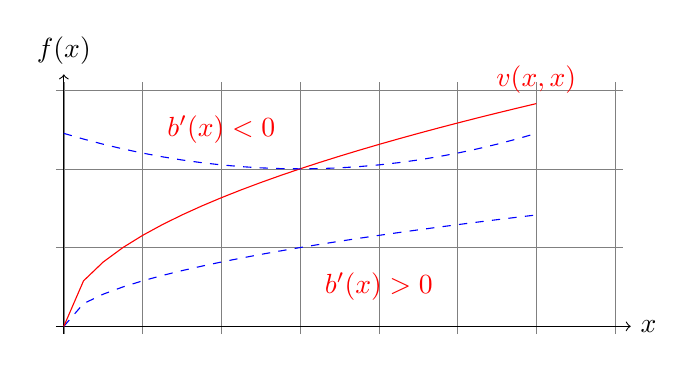
\begin{tikzpicture}[domain=0:6]
    \draw[very thin,color=gray] (-0.1,-0.1) grid (7.1,3.1);
    \draw[->] (-0.1,0) -- (7.2,0) node[right] {$x$};
    \draw[->] (0,-0.1) -- (0,3.2) node[above] {$f(x)$};
    \draw[color=blue, dashed] plot (\x, {sqrt(\x/3)}) ;
    \draw[color=red] plot (\x, {2*sqrt(\x/3)})
        node[above] {$v(x,x)$};
    \draw[color=blue, dashed] plot (\x, {0.05*(\x-3)*(\x-3)+2});
    \node [red] at (2,2.5) {$b'(x)<0$};
    \node [red] at (4,0.5) {$b'(x)>0$};
\end{tikzpicture}



Решения, не удовлетворяющие условию $ b(0)=0 $, обязательно убывают при небольших $ x $. Но наше дифференциальное уравнение является необходимым условием только для случая возрастающей $ b(x) $. Мы пользовались возрастанием функции $ b() $ при исполнении чудо-замены. Только решение,  удовлетворяющее условию $ b(0)=0 $, позволяет оправдать чудо-замену.

Осталось доказать, что решение с начальным условием $ b(0)=0 $ удовлетворяет какому-нибудь достаточному условию максимума. Мы докажем, что знак производной меняется с плюса на минус, как и положено.


Присмотримся повнимательнее к первой производной прибыли.
\begin{multline}
\frac{\partial \pi(x,b(a))}{\partial a}=v(x,a)g(a|x)-b(a)g(a|x)-b'(a)G(a|x)=\\
=(v(x,a)-b(a))g(a|x)-b'(a)G(a|x)=\\
=(v(x,a)-v(a,a)+v(a,a)-b(a))g(a|x)-b'(a)G(a|x)=\\
(v(x,a)-v(a,a))g(a|x)+(v(a,a)-b(a))g(a|x)-b'(a)G(a|x)
%G(a|x)\left((v(x,a)-b(a))R(a|x)-b'(a) \right)
\end{multline}

Функция $ b() $ является решением дифференциального уравнения \ref{b_first_de}, поэтому $ v(a,a)-b(a)=b'(a)/R(a|a) $,

\begin{multline}
\frac{\partial \pi(x,b(a))}{\partial a}=(v(x,a)-v(a,a))g(a|x)+\frac{b'(a)}{R(a|a)}g(a|x)-b'(a)G(a|x)=\\
(v(x,a)-v(a,a))g(a|x)+b'(a)g(a|x)\left(\frac{1}{R(a|a)}-\frac{1}{R(a|x)} \right)
\end{multline}

\begin{enumerate}
\item Рассмотрим $ a>x $. Во-первых, $ v(x,a)<v(a,a) $ так как $ v() $ возрастает по обоим аргументам. Во-вторых, $1/R(a|a)<1/R(a|x) $, поскольку $ R(a|x) $ возрастает по второму аргументу. Значит, справа производная отрицательна.
\item Рассмотрим $ a<x $. Во-первых, $ v(x,a)>v(a,a) $ так как $ v() $ возрастает по обоим аргументам. Во-вторых, $1/R(a|a)>1/R(a|x) $, поскольку $ R(a|x) $ возрастает по второму аргументу. Значит, слева производная положительна.
\end{enumerate}

Кстати, никаких секретов в решении линейных дифференциальных уравнений первого порядка в 21 веке нет, поэтому мы можем его предъявить в явном виде,
\begin{equation}
b(x)=\int_{0}^{x}v(y,y)R(y|y)\cdot \exp\left(-\int_{y}^{x}R(t|t)dt\right) dy
\end{equation}

Можно убедиться, что оно подходит и в само уравнение, и к условию $ b(0)=0 $, или получить его самостоятельно методом вариации постоянной. Но форма его настолько громоздкая, что проще решать задачи без него.
\end{proof}

В качестве побочного результата мы получили доказательство того, что $ b(x)\leq v(x,x) $.

Для последующего сравнения прибыли продавца нам потребуется функция выплат первого игрока. Вероятность того, что первый выиграет аукцион если его сигнал равен $ x $ равна $ \P(Y_{1}<x|X_{1}=x)=G(x|x)$. Поэтому:
\begin{equation}
pay^{FP}(x)=b^{FP}(x)G(x|x)
\end{equation}

Здесь мы обозначили равновесную стратегию не как $ b() $, а как $ b^{FP}() $, так как она отличается от равновесной стратегии на других аукционах.

\item Аукцион второй цены.\index{аукцион!второй цены}

При решении задач мы столкнулись с тем, что аукцион второй цены в каком-то смысле правдивый, то есть ставить надо свою ценность. Когда ценность не совпадает с сигналом верен очень похожий результат:

\begin{myth} \label{NE_SP}
На аукционе второй цены равновесием Нэша будет набор стратегий: $b(x):=v(x,x)=\E(V_{1}|X_{1}=x \cap Y_{1}=x)$.
\end{myth}
\begin{proof}
Пусть остальные игроки используют предлагаемую стратегию, а первый ставит $ b_{1} $.
\begin{equation}
\pi(x,b_{1})=\E((V_{1}-b(Y_{1}))1_{W_{1}}|X_{1}=x; Bid_{1}=b_{1})
\end{equation}

Сделаем замену $ b_{1}=b(a) $, она упрощает нам событие $ W_{1} $ до $ W_{1}=\{Y_{1}<a\} $
\begin{multline}
\pi(x,b(a))=\E((V_{1}-b(Y_{1}))1_{Y_{1}<a}|X_{1}=x)=\\
=\E((V_{1}1_{Y_{1}<a}|X_{1}=x)-\E(b(Y_{1}))1_{Y_{1}<a}|X_{1}=x)
\end{multline}

Отдельно считаем вычитаемое:
\begin{equation}
\E(b(Y_{1}))1_{Y_{1}<a}|X_{1}=x)=\int_{0}^{a}b(y)g(y|x)dy=\int_{0}^{a}v(y,y)g(y|x)dy
\end{equation}

И применив к уменьшаемому формулу \ref{iterated_e}, получаем
\begin{multline}
\E((V_{1}1_{Y_{1}<a}|X_{1}=x)=\int_{0}^{1}\E(V_{1}1_{Y_{1}<a}|X_{1}=x \cap Y_{1}=y)g(y|x)dy=\\
\int_{0}^{a}\E(V_{1}|X_{1}=x \cap Y_{1}=y)g(y|x)dy=\int_{0}^{a}v(x,y)g(y|x)dy
\end{multline}


Значит,
\begin{equation}
\pi(x,b(a))=\int_{0}^{a}(v(x,y)-v(y,y)) g(y|x)dy
\end{equation}

Если $ y<x $, то величина $ v(x,y)-v(y,y)>0 $ в силу того, что $ v(x,y) $ возрастает по $ x $. Мы хотим, максимизировать прибыль, то есть мы хотим интегрировать до тех пор, пока подынтегральное выражение положительно. то есть оптимальное $ a=x $. Остаётся заметить, что по предположению игрок делает ставку $ b_{1}=b(a) $. Но оптимальное $ a=x $, значит, оптимальная ставка равна $ b(x) $.


\end{proof}


Для последующего сравнения прибыли продавца нам потребуется функция выплат первого игрока:
\begin{equation}
pay^{SP}(x)=\E(b(Y_{1})1_{Y_{1}<x}|X_{1}=x)=\int_{0}^{x}v(t,t)g(t|x)dt
\end{equation}





\end{itemize}



\section{Теорема о сравнении доходностей}


\begin{myth}\index{теорема!о сравнении доходностей}
Если:

\begin{enumerate}
\item[RC1.] Сигналы $ X_{i} $ имеют регулярное на $ [0;1] $ распределение
\item[RC2.] Сигналы $ X_{i} $ аффилированы
\item[RC3.] Игроки симметричны, в частности:
\begin{enumerate}
\item[RC3a.] Совместная функция плотности сигналов симметрична
\item[RC3b.] Ценность игрока симметрична относительно сигналов других игроков.
\end{enumerate}
\item[RC4.] Ценность является возрастающей функцией от сигналов, $ u(0,\ldots,0)=0 $.

\end{enumerate}

То:
\begin{equation}
\E(R^{B})\geq \E(R^{SP})\geq \E(R^{FP})
\end{equation}

\end{myth}

\begin{proof}
Сначала докажем, что для продавца аукцион второй цены лучше, чем аукцион первой цены, $\E(R^{SP})\geq \E(R^{FP})$.


Мы снова воспользуемся дифференциальным уравнением \ref{b_first_de}:
\begin{multline}
pay^{SP}(x)=\int_{0}^{x}v(y,y)g(y|x)dy=\\
=\int_{0}^{x}(v(y,y)-b^{FP}(y))g(y|x)dy+\int_{0}^{x}b^{FP}(y)g(y|x)dy=\\
=\int_{0}^{x}b'^{FP}(y)\frac{1}{R(y|y)}g(y|x)dy+\int_{0}^{x}b^{FP}(y)g(y|x)dy=\\
=\int_{0}^{x}b'^{FP}(y)\frac{R(y|x)}{R(y|y)}G(y|x)dy+\int_{0}^{x}b^{FP}(y)g(y|x)dy\geq\\
\geq \int_{0}^{x}b'^{FP}(y)G(y|x)dy+\int_{0}^{x}b^{FP}(y)g(y|x)dy
\end{multline}
Последний переход верен в силу того, что $ y<x $.

А теперь долго и пристально смотрим на эти два интеграла и берём их в уме оба сразу:
\begin{multline}
\int_{0}^{x}b'^{FP}(y)G(y|x)dy+\int_{0}^{x}b^{FP}(y)g(y|x)dy=\\
\int_{0}^{x}b^{FP}(y)g(y|x)+b'^{FP}(y)G(y|x) dy=b^{FP}(x)G(y|x)=pay^{FP}(x)
\end{multline}

Мы сравнили детерминистические функции выплат. А ожидаемый доход продавца связан с ними:
\begin{equation}
\E(R)=n\cdot \E(Pay_{1})=n\cdot \int_{0}^{1}pay(x)f(x) \, dx
\end{equation}
Мы снова применяем трюк с условным подсчётом математического ожидания \ref{conditional_way}.

Теперь докажем, что для продавца кнопочный аукцион лучше, чем аукцион второй цены $ \E(R^{B})\geq \E(R^{SP}) $.

Только для целей этого доказательства введём функцию
\[
z(x,y)=\E(u(Y_{1},Y_{1},\ldots,Y_{n-1})|X_{1}=x,Y_{1}=y).
\]

Напомним её смысл. На кнопочном аукционе самый сильный игрок, за исключением первого игрока, жмёт кнопку до момента $ u(Y_{1},Y_{1},\ldots,Y_{n-1}) $. Именно столько заплатит первый игрок, если выиграет аукцион. По теореме \ref{aff_multi_f} функция $ z(x,y) $ возрастает по обоим аргументам.

Сначала мы замечаем, что $ v(y,y)=z(y,y) $,
\begin{multline}
v(y,y)=\E(V_{1}|X_{1}=y, Y_{1}=y)=\E(u(X_{1},Y_{1},\ldots,Y_{n-1})|X_{1}=y, Y_{1}=y)=\\
=\E(u(Y_{1},Y_{1},\ldots,Y_{n-1})|X_{1}=y, Y_{1}=y)=z(y,y)
\end{multline}

Если $ x>y $, то $ v(y,y)<z(x,y) $. А теперь считаем ожидаемую доходность продавца:
\begin{multline}
\E(R^{SP})=\E(b^{SP}(Y_{1})|X_{1}>Y_{1})=\E(v(Y_{1},Y_{1})|X_{1}>Y_{1})\leq\\
\leq \E(z(X_{1},Y_{1})|X_{1}>Y_{1})
\end{multline}

Заметим, что в правой части написано математическое ожидание от условного математического ожидания в случайной точке. Пользуясь идеей \ref{conditional_way}\index{условное математическое ожидание} мы видим, что:
\begin{equation}
\E(z(X_{1},Y_{1})|X_{1}>Y_{1})=\E(u(Y_{1},Y_{1},\ldots,Y_{n-1})|X_{1}>Y_{1})=\E(R^{B})
\end{equation}

\end{proof}

\section{Задачи}
\begin{enumerate}
\item Аукцион второй цены с резервной ценой\index{аукцион!второй цены с резервной ценой}. Имеется $n$ покупателей.  Сигналы независимы и равномерны на $ [0;1] $, $ V_{i}=X_{i} $. Покупатели одновременно делают ставки. Если наибольшая ставка больше $ r $, то игрок с максимальной ставкой получает товар. Если наибольшая ставка меньше $ r $, то товар остаётся у продавца\index{резервная цена}. Победитель платит продавцу максимум между второй по величине ставкой и $r$.
\begin{enumerate}
\item Найдите равновесие Нэша.
\item Найдите оптимальное $ r $ для продавца, если ценности равномерны на отрезке $ [0;1] $.
\end{enumerate}


\item Аукцион первой цены с резервной ценой $ r $\index{аукцион!первой цены с резервной ценой}. Имеется $ n $ покупателей.  Сигналы независимы и равномерны на $ [0;1] $, $ V_{i}=X_{i} $. Покупатели одновременно делают ставки. Если наибольшая ставка больше $ r $, то игрок с максимальной ставкой получает товар. Если наибольшая ставка меньше $ r $, то товар остаётся у продавца. Победитель платит продавцу свою ставку. Предполагаем, что $ r $ известна покупателям.
\begin{enumerate}
\item Найдите равновесие Нэша.
\item Найдите оптимальное $ r $ для продавца, если ценности равномерны на $ [0;1] $.
\end{enumerate}


\item Аукцион второй цены с платой за вход\index{аукцион!второй цены с платой за вход}. Имеется $ n $ покупателей.  Сигналы независимы и равномерны на $ [0;1] $, $ V_{i}=X_{i} $. Покупатели одновременно решают делать ли ставку, и если делать, то какую. Сделавший ставку платит $ w $ вне зависимости от того, победил ли он. Игрок с максимальной ставкой получает товар. Если ставок не было, то товар остаётся у продавца. Победитель платит продавцу вторую по величине ставку. Если на аукцион вошёл только один игрок, то он побеждает и  ничего кроме платы за вход не платит.
\begin{enumerate}
\item Найдите равновесие Нэша.
\item Найдите оптимальное $ w $ для продавца, если ценности равномерны на $ [0;1] $.
\end{enumerate}


\item Аукцион первой цены с платой за вход\index{аукцион!первой цены с платой за вход}. Имеется $ n $ покупателей.  Сигналы независимы и равномерны на $ [0;1] $, $ V_{i}=X_{i} $. Покупатели одновременно решают делать ли ставку, и если делать, то какую. Сделавший ставку платит $ w $ вне зависимости от того, победил ли он. Игрок с максимальной ставкой получает товар. Если ставок не было, то товар остаётся у продавца. Победитель платит продавцу свою ставку.
\begin{enumerate}
\item Найдите равновесие Нэша.
\item Найдите оптимальное $ w $ для продавца, если ценности равномерны на $ [0;1] $.
\end{enumerate}

\item Верно ли, что $ \E(R) $ одинаково в аукционе первой и второй цены с резервной ценой?

\item Верно ли, что $ \E(R) $ одинаково в аукционе первой и второй цены с платой за вход?

\item Величины $ X_{1} $, $ X_{2} $ и $ X_{3} $ независимы и равномерны на $ [0;1] $. В аукционе второй цены участвуют два игрока: первый знает $ X_{1} $, второй — $ X_{2} $. Ценность товара общая, $ V_{1}=V_{2}=X_{1}+X_{2}+X_{3} $. Найдите равновесие Нэша и ожидаемый доход продавца.

\item По аналогии с определением условной обратной функции риска дайте определение безусловной обратной функции риска\index{безусловная обратная функция риска}, $ R(x) $. Пусть $ X $ — случайная величина, показывающая время в часах, которое я трачу на написание одной лекции. Как можно проинтерпретировать $ R(5)=10 $?
\item Автобусы приходят на остановку согласно пуассоновскому потоку с интенсивностью $ \lambda=6 $ автобусов в час. Вася стоит некоторое время у остановки. Сколько в среднем автобусов приедет за это время? Какова вероятность, что не приедет ни одного автобуса? Рассмотрите два случая:
\begin{enumerate}
\item Вася стоит у остановки ровно 5 минут.
\item Вася стоит у остановки случайное время $ X $ (в минутах), независимое от времени прихода автобусов. Функция плотности $ X $ имеет вид $ f(x)= \frac{x}{25}$ при $ x\in [0;10] $.
\end{enumerate}
Подсказка: Первый пункт — это не что иное, как $ \E(N|X=5) $.
\item Найдите функции $ g(x,y)$, $ g(y|x)$, $ G(y|x)$,  $R(y|x)$ и $v(x,y)$ для случаев:
\label{ex_vxy}
\begin{enumerate}
\item Сигналы независимы, равномерны на $ [0;1] $, $ V_{i}=X_{i} $.
\item Три игрока. Сигналы независимы, равномерны на $ [0;1] $, $ V_{1}=X_{1}+X_{2}X_{3} $.
\item Три игрока. Ценность равна $ V_{1}=X_{1}+X_{2}X_{3} $. Совместная функция плотности сигналов при $ x_{1},x_{2},x_{3}\in[0;1]$ имеет вид \[
f(x_{1},x_{2},x_{3})=7/8+x_{1}x_{2}x_{3}
\].
\end{enumerate}
\end{enumerate}


\section{Решения задач}

\begin{enumerate}
\item Аукцион второй цены с резервной ценой.\index{аукцион!второй цены с резервной ценой}

С помощью таблички доказываем, что игрокам оптимально говорить правду. Конечно, если ценность меньше $ r $, то оптимально говорить любое число ниже $ r $. Но правду оптимально говорить всегда.

Первый игрок в среднем платит:
\begin{equation}
\E(Pay_{1})=r\cdot \P(X_{1}>r>Y_{1})+\E(Y_{1}\cdot 1_{X_{1}>Y_{1}>r})
\end{equation}

Совместная функция плотности $ X_{1} $ и $ Y_{1} $ имеет вид:
\begin{equation}
g(x,y)=(n-1)y^{n-2}
\end{equation}

Значит, первое слагаемое равно:
\begin{equation}
r\P(X_{1}>r>Y_{1})=r\int_{r}^{1}\int_{0}^{r} (n-1)y^{n-2} dy dx=(1-r)r^{n}
\end{equation}

И второе слагаемое равно:
\begin{multline} \label{E_Y_1XYr}
\E(Y_{1}\cdot 1_{X_{1}>Y_{1}>r})=\int_{r}^{1}\int_{r}^{x} y\cdot (n-1)y^{n-2} dy dx=\\
=(n-1)\left(\frac{1}{n(n+1)}-\frac{\rho^{n}}{n}+\frac{\rho^{n+1}}{n+1}\right)
\end{multline}

Значит, средняя выплата первого игрока равна:
\begin{multline}
\E(Pay_{1})=(1-r)r^{n}+(n-1)\left(\frac{1}{n(n+1)}-\frac{r^{n}}{n}+\frac{r^{n+1}}{n+1}\right)=\\
=\frac{r^{n}}{n}-\frac{2r^{n+1}}{n+1}+\frac{n-1}{n(n+1)}
\end{multline}

Максимизируем по $ r $ и находим, что $ r^{*}=0.5 $.


\item Аукцион первой цены с резервной ценой\index{аукцион!первой цены с резервной ценой}. Рассуждаем за первого игрока:

\begin{equation}
\pi_{1}(x,b_{1})=(x-b_{1})\P(b_{1}\geq \max\{b(Y_{1}),r\})
\end{equation}

Наша задача максимизировать эту функцию, выбирая произвольное $ b_{1} $.

Если $ x<r $, то нам ничего не светит, оптимально не участвовать в аукционе, то есть можно делать любую ставку меньше $ r $. Если $ x\geq r $, то оптимально участвовать в аукционе с некоторой ставкой $ r\leq b_{1}\leq x $. В частности, получаем, что $ b(r)=r$.


%Отметим, что максимум ожидаемой прибыли, то есть функция $\pi_{1}(x,b_{1}^{*}(x))$, должна плавно зависеть от $ x $. Действительно, при $ x<r $ максимум прибыли равен нулю. А при $ x=r+\varepsilon $ оптимальная ставка $ b_{1}\in[r;r+\varepsilon] $, поэтому вероятность в формуле прибыли примерно равна нулю.

Предположим, что $ x\geq r $. Тогда целевая функция упростится до старой, без резервной цены!

\begin{equation}
\pi_{1}(x,b_{1})=(x-b_{1})\P(b_{1}\geq b(Y_{1}))
\end{equation}

Делаем вывод. Если $x\geq r$, то оптимальное $ b_{1}(x) $ удовлетворяет старому дифференциальному уравнению.

Напомним, что старое уравнение было
\begin{equation}
b'(x)x=(n-1)(x-b(x))
\end{equation}

И его решением имело вид
\begin{equation}
b(x)=cx^{1-n}+\frac{n-1}{n}x
\end{equation}

На этот раз $ c $ надо искать из условия $ b(r)=r $. Раньше, кстати, начальное условие было $b(0)=0 $. Отсюда находим $ c=r^{n}/n $ и частное решение:
\begin{equation}
b(x)=\frac{r^{n}}{n}x^{1-n}+\frac{n-1}{n}x, \quad x\geq r
\end{equation}

На всякий пожарный можно убедиться, что функция $b(x)$ возрастает по $ x $.

Ожидаемая выплата от первого игрока,
\begin{multline}
\E(b(X_{1})1_{X_{1}\geq Y_{1},X_{1}\geq r})=\int_{r}^{1} \int_{0}^{x} b(x)g(x,y)dy dx =\\
=\int_{r}^{1} b(x) \int_{0}^{x} g(x,y)dy dx =\int_{r}^{1} b(x) \int_{0}^{x} (n-1) y^{n-2} dy dx =\\
=\int_{r}^{1}b(x) x^{n-1} dx=\frac{r^{n}}{n}-\frac{2r^{n+1}}{n+1}+\frac{n-1}{n(n+1)}
\end{multline}

Зависимость выплаты первого игрока от $ r $ такая же, как на аукционе второй цены.


\item Аукцион второй цены с платой за вход.\index{аукцион!второй цены с платой за вход}

%На аукционе второй цены с резервной ценой $ r $ реально играют только игроки с ценностью выше $ r $.

Для начала заметим, что если игрок решил делать ставку, то ему оптимально делать ставку, равную ценности. Доказательство стандартное, стратегия $ b_{1}=X_{1} $ нестрого доминирует все остальные. Осталось определить, при каких $ X_{1} $ первому игроку лучше играть, а при каких  — нет.

Предполагаем, что оптимальная стратегия имеет вид: если $ x\geq \rho $, то делать ставку $ b_{1}=x $, если $ x<\rho $, то не делать ставку. Предположим кроме того, что равновесные стратегии $ b(x) $ возрастают по $ x $ при $ x\geq \rho $.
%Не участие в аукционе мы можем кодировать например, как $ b(x)=0 $ при $ x<\rho $.

Рассмотрим игрока с ценностью $ x\geq \rho $ в равновесии Нэша. Какова вероятность того, что он выиграет аукцион? Поскольку $ b(x) $ монотонно возрастает вероятность выигрыша по-прежнему:
\begin{equation}
q(x)=F^{n-1}(x),\quad x\geq \rho
\end{equation}

Игрок с ценностью $ \rho $ должен быть безразличен между ставкой $ b(\rho) $ и не участием в аукционе. Не участвуя в аукционе, он получает ноль. Участвуя, он выиграет только если все остальные не участвуют, то есть он выигрывает аукцион по нулевой цене. Значит, условие безразличия имеет вид:
\begin{equation}
-w+\rho F^{n-1}(\rho)=0
\end{equation}

Применительно к нашему случаю $ F(x)=x $ получаем $ \rho=w^{1/n} $.


Ожидаемая выплата от первого игрока равна:

\begin{multline}
\E(Pay_{1})=\E(Y_{1}1_{X_{1}>Y_{1}>\rho})+w\P(X_{1}>\rho)=\\
=\E(Y_{1}1_{X_{1}>Y_{1}>\rho})+w(1-\rho)
\end{multline}

Первое слагаемое мы уже искали, см. \ref{E_Y_1XYr}:
\begin{equation}
\E(Y_{1}1_{X_{1}>Y_{1}>\rho})=(n-1)\left(\frac{1}{n(n+1)}-\frac{\rho^{n}}{n}+\frac{\rho^{n+1}}{n+1}\right)
\end{equation}

Складываем, и, как и раньше получаем:
\begin{multline}
\E(Pay_{1})=(n-1)\left(\frac{1}{n(n+1)}-\frac{\rho^{n}}{n}+\frac{\rho^{n+1}}{n+1}\right)+\rho^{n}(1-\rho)=\\
=\frac{\rho^{n}}{n}-\frac{2\rho^{n+1}}{n+1}+\frac{n-1}{n(n+1)}
\end{multline}

\item Аукцион первой цены с платой за вход.\index{аукцион!первой цены с платой за вход}

Предположим, что оптимальная стратегия имеет вид: Если $ x\geq \rho $, то делать ставку $ b(x) $; если $ x<\rho $, то не делать ставку. Предположим, что эта $ b() $ возрастающая при $ x\geq \rho $. Как и на аукционе второй цены из этого следует, что вероятность выигрыша первого игрока при $ x\geq\rho $ равна:
\begin{equation}
q(x)=F(x)^{n-1}=x^{n-1}
\end{equation}


Если $ x=\rho $, то игроку должно быть безразлично, делать или не делать ставку. Если ему не безразлично, то значит, $ \rho $ выбрано не оптимально. Ожидаемый выигрыш первого игрока при ценности $ \rho $:
\begin{equation}
(\rho-b(\rho))F(\rho)^{n-1}-w=0
\end{equation}

Заметим, что $ b(\rho)=0 $. Действительно, игрок с пороговой ценностью $ \rho $ может выиграть только если у остальных ценность ниже $ \rho $, то есть если остальные не участвуют. А при таком условии победы оптимально ставить $ b(\rho)=0 $.

Получаем такой же порог участия как на аукционе второй цены,
\begin{equation}
\rho=w^{1/n}
\end{equation}

Рассматриваем случай $ x\geq \rho $. В этом случае прибыль совпадает со старой. Мы получаем старое дифференциальное уравнение и старое решение
\begin{equation}
b(x)=cx^{1-n}+\frac{n-1}{n}x
\end{equation}

И начальное условие $ b(\rho)=0 $. Получаем $ c=\frac{1-n}{n}\rho^{n} $ и частное решение
\begin{equation}
b(x)=\frac{n-1}{n}x(1-\rho^{n}x^{-n})
\end{equation}

Считаем ожидаемый платеж первого игрока,
\begin{equation}
\E(Pay_{1})=\E(b(X_{1})1_{X_{1}\geq Y_{1},X_{1}\geq \rho})+\rho^{n}\P(X_{1}>\rho)
%\int_{\rho}^{1}\int_{0}^{x} \frac{n-1}{n}x(1-\rho^{n}x^{-n}) g(x,y) dy dx+\rho^{n}(1-\rho)=\ldots=\\
%\frac{\rho^{n}}{n}-\frac{2\rho^{n+1}}{n+1}+\frac{n-1}{n(n+1)}
\end{equation}

Первый интеграл,
\begin{multline}
\E(b(X_{1})1_{X_{1}\geq Y_{1},X_{1}\geq \rho})=\int_{\rho}^{1} \int_{0}^{x} b(x)g(x,y)dy dx =\\
\int_{\rho}^{1} b(x) \int_{0}^{x} g(x,y)dy dx =\int_{\rho}^{1} b(x) \int_{0}^{x} (n-1) y^{n-2} dy dx =\\
\int_{\rho}^{1}b(x) x^{n-1} dx=(n-1)\left(\frac{1}{n(n+1)}-\frac{\rho^{n}}{n}+\frac{\rho^{n+1}}{n+1}\right)
\end{multline}

В сумме, как и раньше,
\begin{equation}
\E(Pay_{1})=\frac{\rho^{n}}{n}-\frac{2\rho^{n+1}}{n+1}+\frac{n-1}{n(n+1)}
\end{equation}

\item  Верно ли, что $ \E(R) $ одинаково в аукционе первой и второй цены с резервной ценой? Да.

\item  Верно ли, что $ \E(R) $ одинаково в аукционе первой и второй цены с платой за вход? Да.

Более того, можно заметить, что аукцион с резервной ценой $ r $ похож на аукцион с платой за вход $ w=r\cdot F(r)^{n-1} $.

\item %Величины $ X_{1} $, $ X_{2} $ и $ X_{3} $ независимы и равномерны на $ [0;1] $. В аукционе второй цены участвуют два игрока: первый знает $ X_{1} $, второй — $ X_{2} $. Ценность товара общая, $ V_{1}=V_{2}=X_{1}+X_{2}+X_{3} $. Найдите равновесие Нэша и ожидаемый доход продавца.
Можно воспользоваться теоремой \ref{NE_SP} и сказать, что равновесная стратегия имеет вид
\begin{multline}
b(x)=\E(V_{1}|X_{1}=x,Y_{1}=x)=\\
=\E(X_{1}+X_{2}+X_{3}|X_{1}=x,Y_{1}=x)=x+\E(X_{2}+X_{3}|Y_{1}=x)
\end{multline}

Внимание! Здесь есть небольшая ловушка! Игроков всего два! Величина $X_{3} $ — это не сигнал от Природы третьему игроку! Величина $ X_{3} $ — это просто составляющая ценности, неизвестная обоим игрокам. Поэтому здесь $ Y_{1}=X_{2} $, а не $ Y_{1}=\max\{X_{2},X_{3}\} $. Остаётся вспомнить про независимость $ X_{2} $ и $ X_{3} $ и получить:
\begin{multline}
x+\E(X_{2}+X_{3}|Y_{1}=x)=x+\E(X_{2}+X_{3}|X_{2}=x)=\\
=x+x+\E(X_{3})=2x+0.5
\end{multline}

Считаем ожидаемый выигрыш продавца,
\begin{equation}
\E(R)=2\E(\min\{X_{1},X_{2}\})+0.5=2\int_{0}^{1}y\cdot 2(1-y)dy+0.5=\ldots=\frac{7}{6}
\end{equation}

%Интуитивно. Во-первых, $ Y_{2}<x$. Во-вторых, $ Y_{2} $ когда-то раньше была одним из $ X_{i} $, то есть была равномерной на $ [0;1] $. Значит, $ \E(Y_{2}|Y_{1}=x)=x/2 $. Итого: $ b(x)=2.5x $.

\item Обратная функция риска\index{безусловная обратная функция риска}, $ R(x)=f(x)/F(x) $, где $ f() $ — функция плотности, а $ F() $ — функция распределения случайной величины $ X $. Пусть $ X $ — случайная величина, показывающая время в часах, которое я трачу на написание одной лекции. Проинтерпретировать $ R(5)=10 $ можно с помощью небольшой $ \Delta=0.01 $ (одна сотая часа — это 36 секунд). Если известно, что прошло 5 часов после начала написания лекций, и я уже отдыхаю, то вероятность того, что я их окончил за только что истёкшие 36 секунд, примерно равна $ R(5)\cdot \Delta=0.1 $.
\item Обозначим $ N$ — количество пришедших автобусов, а $ X $ — время, которое Вася наблюдал за остановкой.
\begin{enumerate}
\item Количество автобусов за $ x $ минут имеет распределение Пуассона с параметром $ \lambda_{x}=0.1x $, так как в среднем 6 автобусов в час, это в среднем 0.1 автобуса в минуту. $ \E(N|X=5)=0.5 $
\item \begin{equation} \E(N)=\int_{0}^{10}\E(N|X=x)f(x)dx=\int_{0}^{10}0.1x\cdot \frac{x}{25} dx=\frac{4}{3} \end{equation}
\end{enumerate}
\item Найдите функции $ g(x,y)$, $ g(y|x)$, $ G(y|x)$,  $R(y|x)$ и $v(x,y)$ для случаев:
\begin{enumerate}
\item Сигналы независимы, равномерны на $ [0;1] $, $ V_{i}=X_{i} $.
Применяя метод о-малых, находим:
\begin{equation}
g(x,y)=(n-1)y^{n-2}
\end{equation}
\begin{equation}
g(y|x)=g(x,y)/f(x)=(n-1)y^{n-2}
\end{equation}
\begin{equation}
G(y|x)=\int_{0}^{y}(n-1)t^{n-2}dt=y^{n-1}
\end{equation}
\begin{equation}
R(y|x)=\frac{n-1}{y}
\end{equation}
\begin{equation}
v(x,y)=\E(X_{1}|X_{1}=x,Y_{1}=y)=x
\end{equation}

\item Три игрока. Сигналы независимы, равномерны на $ [0;1] $, $ V_{1}=X_{1}+X_{2}X_{3} $.
Отличается только $ v(x,y) $:
\begin{multline}
v(x,y)=\E(X_{1}+X_{2}X_{3}|X_{1}=x,Y_{1}=y)=x+\E(X_{2}X_{3}|Y_{1}=y)=\\
x+\E(Y_{1}Y_{2}|Y_{1}=y)=x+y\E(Y_{2}|Y_{1}=y)
\end{multline}

Здесь мы посчитаем интуитивно, а в следующем пункте — через интегралы. Итак: если я знаю, что $ Y_{1} $, максимум из $ X_{2} $ и $ X_{3} $, равен $ y $, то оставшаяся величина $ Y_{2} $ где-то на отрезке $[0;y] $. Поскольку безусловное распределение было равномерным, то и условное будет равномерным. И условное среднее будет равно $ y/2 $. то есть $ v(x,y)=x+y^{2}/2 $.


\item

\begin{equation}
g(x,y)=2!\cdot \int_{0}^{y} 7/8+x\cdot y\cdot x_{3} dx_{3}=\ldots=\frac{7}{4}y+xy^{3}
\end{equation}

\begin{multline}
g(y|x)=\frac{g(x,y)}{f(x)}=\frac{\frac{7}{4}y+xy^{3}}{\int_{0}^{1}\int_{0}^{1} \frac{7}{8}+xx_{2}x_{3}dx_{2}dx_{3}}=\ldots\\
=\frac{\frac{7}{4}y+xy^{3}}{\frac{7}{8}+\frac{x}{4}}=\frac{14y+8xy^{3}}{7+2x}
\end{multline}

Интегрируя находим:
\begin{equation}
G(y|x)=\int_{0}^{1} g(t|x) dt=\ldots=\frac{7y^{2}+2xy^{4}}{7+2x}
\end{equation}

И взяв отношение:
\begin{equation}
R(y|x)=\frac{g(y|x)}{G(y|x)}=\frac{14y+8xy^{3}}{7y^{2}+2xy^{4}}=\frac{14+8xy^{2}}{7y+2xy^{3}}
\end{equation}

Аналогично предыдущему пункту,
\begin{equation}
v(x,y)=\ldots=x+y\E(Y_{2}|Y_{1}=y)
\end{equation}



Находим совместную функцию плотности величин $ X_{2} $ и $ X_{3} $,
\begin{equation}
f(x_{2},x_{3})=\int_{0}^{1} 7/8+x_{1}\cdot x_{2}\cdot x_{3} dx_{1}=\frac{7}{8}+\frac{1}{2}x_{2}x_{3}, \quad x_{2},x_{3}\in [0;1]
\end{equation}

Из этого сразу следует совместная функция плотности для $ Y_{1} $ и $ Y_{2} $,
\begin{equation}
f_{Y_{1},Y_{2}}(y_{1},y_{2})=2! f(y_{1},y_{2})=\frac{7}{4}+y_{1}y_{2}, \quad 0<y_{2}<y_{1}<1
\end{equation}

И функцию плотности для $ Y_{1} $:
\begin{equation}
f_{Y_{1}}(y_{1})=2!\int_{0}^{y_{1}} f(y_{1},x_{3}) dx_{3}=\ldots=\frac{7}{4}y_{1}+\frac{1}{2}y_{1}^{3}
\end{equation}

Далее находим условную функцию плотности,
\begin{equation}
 f_{Y_{2}|Y_{1}}(y_{2}|y_{1})=\frac{f_{Y_{1},Y_{2}}(y_{1},y_{2})}{f_{Y_{1}}(y_{1})}=\frac{\frac{7}{4}+y_{1}y_{2}}{\frac{7}{4}y_{1}+\frac{1}{2}y_{1}^{3}}, \quad 0<y_{2}<y_{1}<1
\end{equation}

И условное ожидание,
\begin{equation}
\E(Y_{2}|Y_{1}=y)=\int_{0}^{y} y_{2} \frac{\frac{7}{4}+yy_{2}}{\frac{7}{4}y+\frac{1}{2}y^{3}}dy_{2}=\frac{8 \, y^{4} + 21 \, y^{2}}{6 \, {\left(2 \, y^{3} + 7 \, y\right)}}
\end{equation}
И, наконец,
\begin{equation}
v(x,y)=x+\frac{8 \, y^{4} + 21 \, y^{2}}{6 \, {\left(2 \, y^{2} + 7\right)}}
\end{equation}

\end{enumerate}
\end{enumerate}
